\section{Результаты}
\label{sec:conclusion-future}

Тестирование эффективности производилось на примерах и тестах из официального
репозитория ispc. Были выбраны следующие тесты: examples/xpu/mandel,
examples/xpu/aobench, examples/xpu/sgemm, tests/transcendentials-1-1,
tests/varying-float-sqrt. mandel и aobench запускались со следующими
параметрами: \texttt{mandelbrot --scale=16}, и \texttt{aobench 512 512}.
Остальные тесты запускались без дополнительных параметров. На рисунке
~\ref{fig:results} представлено ускорение исполнения выбранных тестовых образцов
в процентах.

\begin{figure}[h]
  \centering
  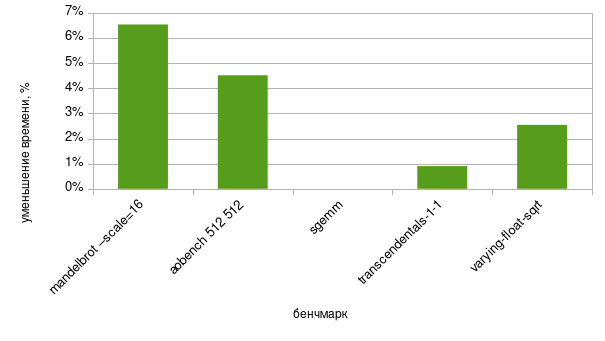
\includegraphics[scale=0.80]{Images/this_graph_explains_everything.png}
  \caption{Результаты замера ускорения исполнения тестовых образцов, %}
  \label{fig:results}
\end{figure}
